
% ----------------------- TODO ---------------------------
% Change per hand-in
\newcommand{\NUMBER}{1} % exercise set number
\newcommand{\EXERCISES}{5} % number of exercises

\newcommand{\COURSECODE}{AP3252}
\newcommand{\TITLE}{EDP indexing}
\newcommand{\STUDENTA}{Jeroen Sangers}
\newcommand{\DEADLINE}{DEADLINE}
\newcommand{\COURSENAME}{Electron Microscopy: Characterisation of the nanoscale}
% ----------------------- TODO ---------------------------

\documentclass[a4paper]{scrartcl}

\usepackage[utf8]{inputenc}
\usepackage[british]{babel}
\usepackage{amsmath}
\usepackage{siunitx}
\usepackage{amssymb}
\usepackage{fancyhdr}
\usepackage{color}
\usepackage{graphicx}
\usepackage{lastpage}
\usepackage{listings}
\usepackage{tikz}
\usepackage{pdflscape}
\usepackage{subfigure}
\usepackage{float}
\usepackage{polynom}
\usepackage{hyperref}
\usepackage{tabularx}
\usepackage{forloop}
\usepackage{geometry}
\usepackage{listings}
\usepackage{fancybox}
\usepackage{tikz}
\usepackage{algpseudocode,algorithm,algorithmicx}
\usepackage{fontspec}


\setmainfont{Baskerville Light}[
	BoldFont	= Baskerville Bold ,
	ItalicFont	= Baskerville Light-Italic
]


% Algorithm command
\newcommand*\Let[2]{\State #1 $\gets$ #2}

% Matrix notation
\newcommand{\matr}[1]{\mathbf{#1}}

% Margins
\geometry{a4paper,left=3cm, right=3cm, top=3cm, bottom=3cm}

% Header and footer setup
\pagestyle {fancy}
%\fancyhead[L]{Tutor: \TUTOR}
\fancyhead[L]{\TITLE}
\fancyhead[C]{\STUDENTA}
\fancyhead[R]{\today}

\fancyfoot[L]{\COURSECODE}
\fancyfoot[C]{\COURSENAME}
\fancyfoot[R]{Page \thepage /\pageref*{LastPage}}

% Formatting of "title"
\def\header#1#2{
  \begin{center}
    {\Large Exercise set}\\
    {(Deadline #2)}
  \end{center}
}

\begin{document}
\subsection*{Silicon sample}
\begin{figure}[H]
  \centering
  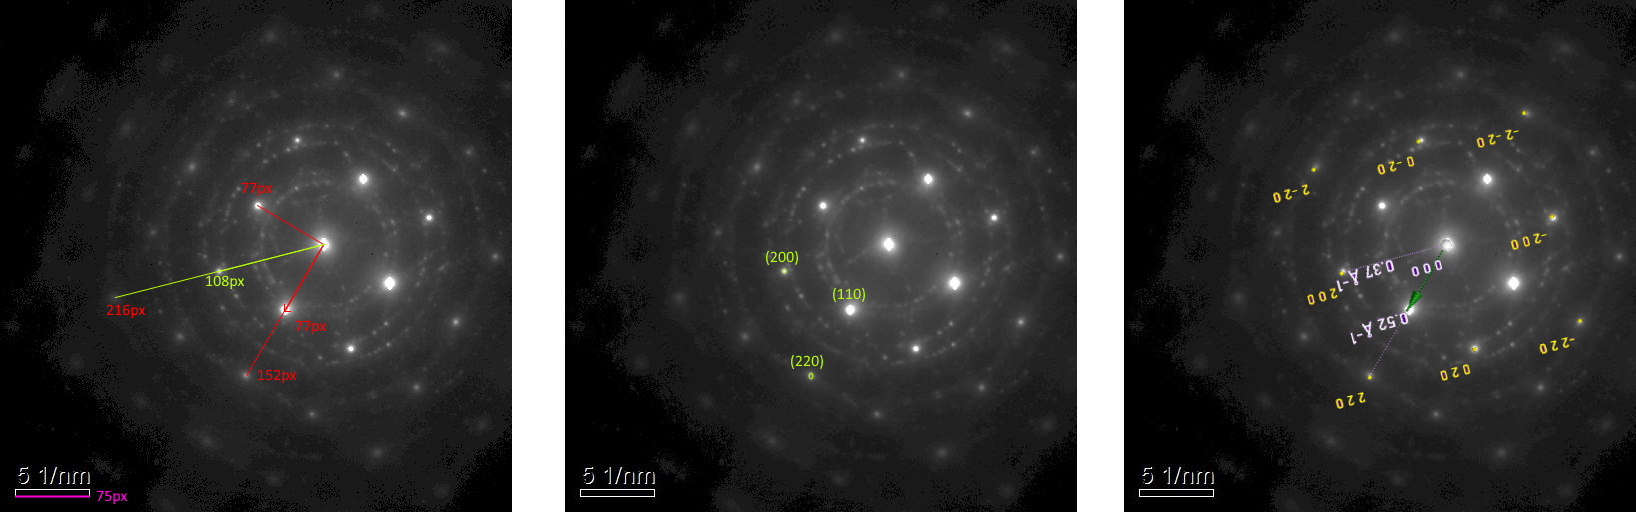
\includegraphics[width=1\linewidth, keepaspectratio]{SI-EDP-index.png}
  \caption{From leftmost to rightmost: A picture with the pixel measurements denoted, A picture with the recognized peaks, A picture with the other peaks overlaid.}
  \label{fig:si_sample}
\end{figure}

\begin{table}[H]
  \centering
  \begin{tabular}{lllllll}
    \textbf{num}           & $|g|$ [$px$] & $|g|$ [$nm^{-1}$] & $d=\frac{2}{g}$ [$nm$] & $d$ [A] & \textbf{angle}          & \textbf{hkl} \\ \hline
    \multicolumn{1}{l|}{0} & 77           & 5.13              & 0.39                   & 3.90    & \multicolumn{1}{l|}{0}  &              \\
    \multicolumn{1}{l|}{1} & 108          & 7.20              & 0.28                   & 2.78    & \multicolumn{1}{l|}{45} & 2 0 0        \\
    \multicolumn{1}{l|}{2} & 77           & 5.13              & 0.39                   & 3.90    & \multicolumn{1}{l|}{90} &              \\
    \multicolumn{1}{l|}{3} & 152          & 10.13             & 0.20                   & 1.97    & \multicolumn{1}{l|}{}   & 2 2 0
  \end{tabular}
  \captionof{table}{Table shows the measurements of the $|\vec{g}|$ in pixels and nanometres and the calculated plane separation in angstrom {\fontfamily{cmr} \AA}. Such that the zone axis is ($004$)}
  \label{tab:si}
\end{table}
\begin{table}[H]
  \centering
  \begin{tabular}{lll}
    \textbf{hkl} & $2/d_{hkl}$ & $d_{hkl}$  [A] \\
    1. 1. 1.     & 6.38        & 3.14           \\
    2. 0. 0.     & 7.36        & 2.72           \\
    2. 2. 0.     & 10.42       & 1.92
  \end{tabular}
  \captionof{table}{Table shows the Eje-Z data for silicon.}
  \label{tab:si_lit}
\end{table}\\

The method for indexing the diffraction pattern was as follows. Firstly the file was loaded into an image editing program, in my case paint.net, after which lines between the centre diffraction spot (000) and three other diffraction spots were drawn, and the pixel lengths were counted. Secondly with the scale bar the pixel values could be converted to nanometres and angstroms. Using these values the (200) and (220) peaks could be identified after which lastly the other diffraction peaks were lined up with the ones identified.
The zone axis was determined to be $(004) = (200) \times (220)$.
\newpage

\begin{figure}
  \centering
  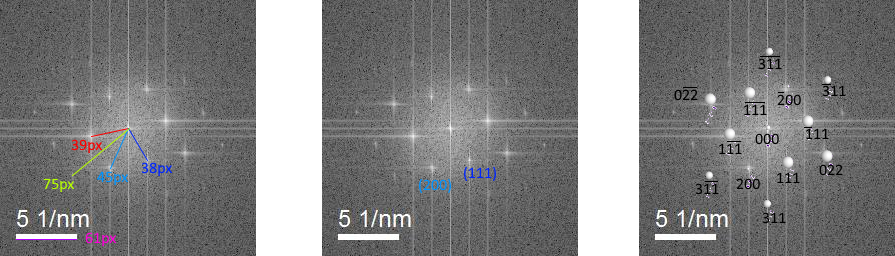
\includegraphics[width=1\linewidth, keepaspectratio]{GaAs-EDP-index.png}
  \caption{From leftmost to rightmost: A picture with the pixel measurements denoted, A picture with the recognized peaks, A picture with the other peaks overlaid.}
\end{figure}

\subsection*{Galiumarsenide sample}
\begin{table}[H]
  \centering
  \begin{tabular}{lllllll}
    \textbf{num} & $|g|$ [$px$] & $|g|$ [$nm^{-1}$] & $d=\frac{2}{g}$ [$nm$] & $d$ [A] & \textbf{angle} & \textbf{hkl}    \\ \hline
    0            & 38           & 3.11              & 0.32                   & 3.21    &                & 1 1 1 or 1 1 -1 \\
    1            & 45           & 3.69              & 0.27                   & 2.71    &                & 2 0 0           \\
    2            & 39           & 3.20              & 0.31                   & 3.13    &                &                 \\
    3            & 75           & 6.15              & 0.16                   & 1.63    &                & 1 1 -3 or 3 1 1
  \end{tabular}
  \captionof{table}{Table shows the measurements of the $|\vec{g}|$ in pixels and nanometres and the calculated plane separation in angstrom {\fontfamily{cmr} \AA}. Such that the zone axis is ($022$). The angles were not calculated since this data was unavailable in Eje-z and rodius was itself unavailable. }
  \label{tab:gaas-lit}
\end{table}
\begin{table}[H]
  \centering
  \begin{tabular}{lll}
    \textbf{hkl} & $2/d_{hkl}$ & $d_{hkl}$  [A] \\
    1. 1. 1.     & 6.13        & 3.26           \\
    1. 1. -1.    & 6.13        & 3.26           \\
    2. 0. 0.     & 7.08        & 2.83           \\
    2. 2. 0.     & 10.01       & 2.00           \\
    1. 1. -3.    & 11.74       & 1.70           \\
    3. 1. 1.     & 11.74       & 1.70
  \end{tabular}
\end{table}

The method for indexing the diffraction pattern was as follows. Firstly the file was loaded into an image editing program, in my case paint.net, after which lines between the centre diffraction spot (000) and three other diffraction spots were drawn, and the pixel lengths were counted. Secondly with the scale bar the pixel values could be converted to nanometres and angstroms. Using these values the (200) and (111) peaks could be identified after which lastly the other diffraction peaks were lined up with the ones identified.
The zone axis was determined to be $(022) = (200) \times (111)$.


\end{document}